\documentclass{article}

% Язык документа
\usepackage[russian]{babel}

% Размеры страницы, отступы
\usepackage[a4paper,top=2cm,bottom=2cm,left=3cm,right=3cm,marginparwidth=1.75cm]{geometry}

% Пакеты
\usepackage{amsmath}
\usepackage{graphicx}
\usepackage[colorlinks=true, allcolors=blue]{hyperref}

\DeclareMathOperator\rot{rot}
\DeclareMathOperator\diver{div}
\DeclareMathOperator\grad{grad}
%----------------------------------------
\begin{document}


\title{Your Paper}
\author{Student}


\maketitle

\begin{abstract}
Your abstract.
\end{abstract}

\tableofcontents{}

\section{Введение}
To view tutorials, user guides, and further documentation, please visit our \href{https://www.overleaf.com/learn}{help library}, or head to our plans page to \href{https://www.overleaf.com/user/subscription/plans}{choose your plan}.

\TeX - это система компьютерной верстки. Набор расширений для системы компьютерной вёрстки \TeX - это \LaTeX, который облегчает набор сложных документов. \LaTeX также можно назвать издательской системой на базе \TeX. В основе работы лежит парадигма редактирования WYSIWYM (What You See Is What You Mean; что вижу, то и подразумеваю), которая является альтернативой WYSIWYG (What You See Is What You Get; используется).

\subsection*{Как работать с \LaTeX?}
Необходимо установить дистрибутив содержащий наборы программ и пакетов (компиляторы, макропакеты, шрифты и т.д.), например TeX Live или MiKTeX. 

\textbf{Программы для редактирования}: TeXmaker, LyX, TeXstudio, TeXworks и т.д.

\textbf{Онлайн редакторы}: Overleaf, Papeeria и др.

\section{Это section}
Здесь можем писать все, что хотим

\subsection{Это subsection}
 Здесь тоже. Добавим новый
 \par
 параграф. А теперь просто перенесем строку (без красной строки)
 \\
 вот так. Если пропустить строку, то эффект будет как от par:
 
"Simply use the section and subsection commands, as in this example document! With Overleaf, all the formatting and numbering is handled automatically according to the template you've chosen. If you're using Rich Text mode, you can also create new section and subsections via the buttons in the editor toolbar."

\subsubsection*{Это subsubsection}
\textbf{Звездочка} убирает \underline{отображение} \textit{нумерации}

\subsection{Изображения}

Это ссылка на лягушку \ref{fig:frog}

\begin{figure}
\centering
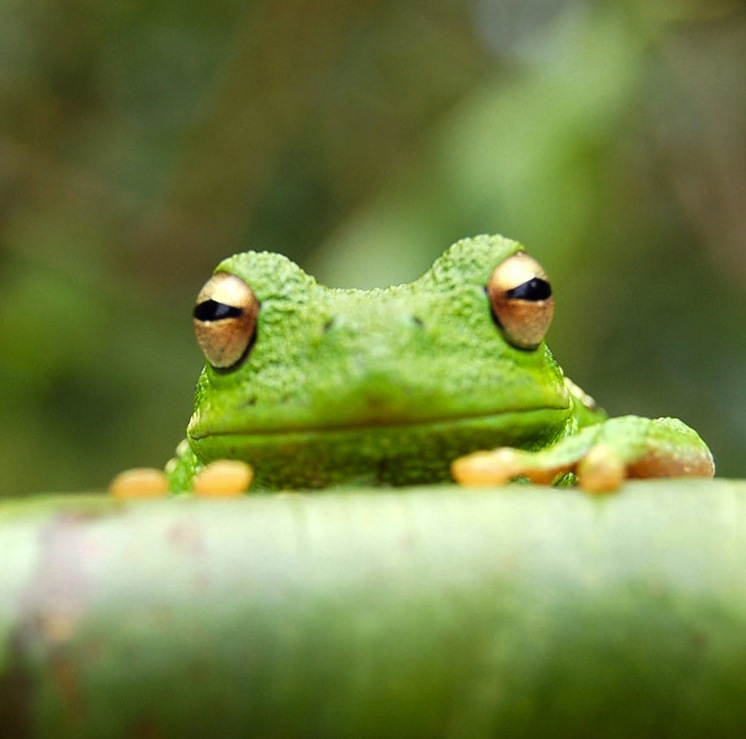
\includegraphics[width=0.3\textwidth]{frog.jpg}
\caption{\label{fig:frog}This frog was uploaded via the file-tree menu.}
\end{figure}

\subsection{Добавление таблиц}

Use the table and tabular environments for basic tables --- see Table~\ref{tab:widgets}, for example. For more information, please see this help article on \href{https://www.overleaf.com/learn/latex/tables}{tables}. 

\begin{table}
\centering
\begin{tabular}{l|r}
Item & Quantity \\\hline
Widgets & 42 \\
Gadgets & 13
\end{tabular}
\caption{\label{tab:widgets}An example table.}
\end{table}

\subsection{Списки}

Можно использовать автоматическую нумерацию

\begin{enumerate}
\item Like this,
\item and like this.
\end{enumerate}
а можно делать неупорядоченные списки
\begin{itemize}
\item Like this,
\item and like this.
\end{itemize}

\subsection{Математика}
Формулы в тексте: $\ddot{\theta}+\omega_0^2 sin(\theta)+2\delta\dot{\theta}=0$
Нумерованная формула:
\begin{equation}
\rho\frac{\partial^{2}U_{i}}{\partial t^{2}}=C_{ijkl}\frac{\partial^{2}U_{l}}{\partial x_{j}\partial x_{k}},\label{eq_label}
\end{equation}
Можно делать ссылку на формулу \ref{eq_label}.

Системы уравнений
\begin{equation}
\begin{cases}
\rot\textbf{E}=-\frac{1}{c}\frac{\partial\textbf{H}}{\partial t},\\
\diver\textbf{H}=0,
\end{cases}\begin{cases}
\rot\textbf{H}=\frac{1}{c}\frac{\partial\textbf{D}}{\partial t},\\
\diver\textbf{E}=0.
\end{cases}\label{max}
\end{equation}


\subsection*{Можно делать ссылки на книги, статьи из .bib файла}
Здесь немного информации от разработчиков:

You can simply upload a \verb|.bib| file containing your BibTeX entries, created with a tool such as JabRef. You can then cite entries from it, like this: \cite{greenwade93}. Just remember to specify a bibliography style, as well as the filename of the \verb|.bib|. You can find a \href{https://www.overleaf.com/help/97-how-to-include-a-bibliography-using-bibtex}{video tutorial here} to learn more about BibTeX.


\bibliographystyle{alpha}
\bibliography{sample}

\end{document}